\section{A 1D quasicrystal: the Fibonacci chain}
\subsection{Dummy}
\begin{frame}{Constructing the Fibonacci chain}
\(
\<{7cm}{\textbf{Fibonacci words}}

Concatenate two words to get the next:
\begin{align*}
	C_0 &= \B \\
	C_1 &= \A \\
	C_2 &= C_1C_0 = \lett{AB} \\
	C_3 &= C_2 C_1 = \lett{ABA} \\
	C_4 &= C_3 C_2 = \lett{ABAAB} \\
	&\vdots
\end{align*}
\[
	C_{l+2} = C_{l+1}C_l
\]
\>
\<{7cm}{\textbf{Properties of Fibonacci words}}
\begin{itemize}
	\item Number of letters follows the Fibonacci sequence:
	
	$\# \A \text{ in } C_{1,2,3,4,\dots} = 1,1,2,3,5,\dots$
	\item 
	$\# \A / \# \B \simop{l\to\infty} \tau$, where $\tau \simeq 1.61$ is the golden ratio.
	\item $\tau$ irrational $\to$ infinite word \textbf{aperiodic}
\end{itemize}
\>
\)
\end{frame}

% counter has to be defined outside of the frame, otherwise a new counter is created at each iteration of only
\newcounter{slideno}
\begin{frame}{Fibonacci word from above}
(Infinite) Fibonacci word: \ca\cb\ca\ca\cb\ca\cb\ca\ca\cb\ca\ca\cb\dots

\ca{} $\leftrightarrow$ horizontal step, \cb{} $\leftrightarrow$ vertical step

\centering
\forloop{slideno}{1}{\value{slideno} < 14}{%
\only<\theslideno>{\includegraphics[width=.7\textwidth]{img/2_part1/CP_fibo_\theslideno}}%
}
\end{frame}

\begin{frame}{Quasiperiodicity of the Fibonacci word}
\(
\<{9cm}
\centering
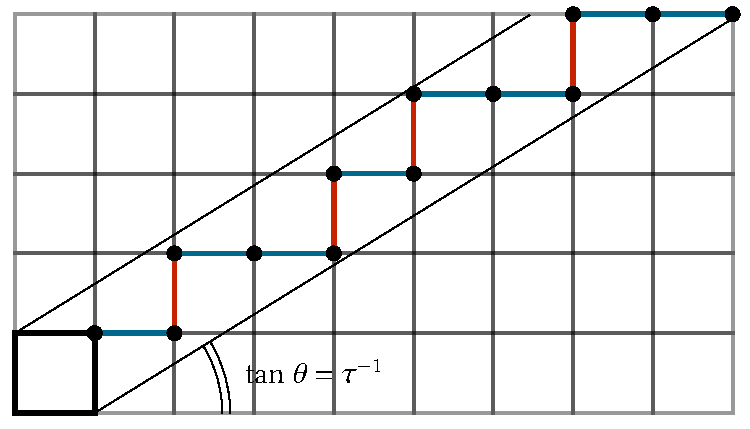
\includegraphics[width=1.\textwidth]{img/2_part1/CP_fibo_cut}
\>
\<{6cm}
\begin{itemize}
	\item average slope = inverse of the golden ratio ($\tau \simeq 1.6$)
	\item bounded fluctuations
\end{itemize}
$\to$ similar environments everywhere

$\to$ quasiperiodicity [Duneau, Katz 85]
\>
\)
\end{frame}

\begin{frame}{Cut-and-project illustrated in the 1D case}
\cp{}: general method to construct quasiperiodic tilings

\(
\<{9cm}
\centering
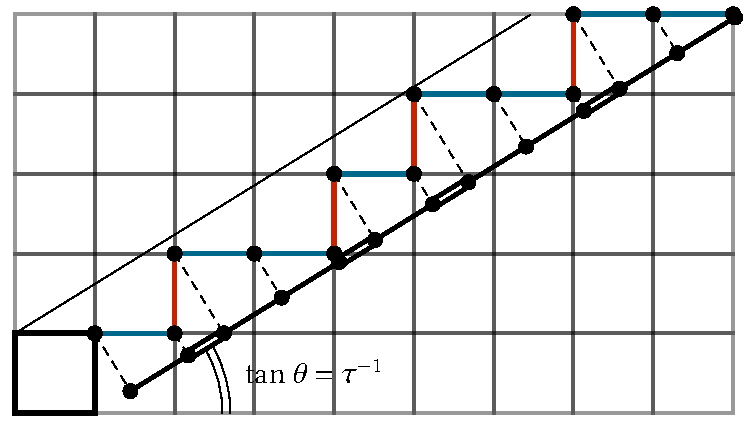
\includegraphics[width=1.\textwidth]{img/2_part1/full_cp}
\>
\<{6cm}
The cut-and-project algorithm:
\begin{enumerate}
	\item choose a hypercubic lattice (here $\zahl^2$)
	\item choose a ``physical plane'' $E_\parallel$ (here a slope)
	\item select points by translating the unit hypercube along $E_\parallel$
	\item project them onto $E_\parallel$.
\end{enumerate}
\>
\)

\end{frame}

\begin{frame}{From letters to atoms}
\begin{itemize}
	\item The Fibonacci word:
	\ca\cb\ca\ca\cb\ca\cb\ca\dots
	
	\item The Fibonacci (tight-binding) chain of atoms:
	
	{\centering
	%\documentclass[draft.tex]{subfiles}
%\documentclass{standalone}
%\usepackage{tikz}
%\begin{document}


    	\begin{tikzpicture}[scale=.6]
    		\newcommand{\orig}{-1.5}
    		\newcommand{\trans}{1.5}
    		\newcommand{\vertspac}{-2.}    		
    		\newcommand{\rad}{2pt} % radii of the circles
    		
    		% set the style of the strong bonds
    		\tikzset{
    			strong/.style={
    				double,
    				double distance=\rad,
    				line width=0.5pt
    				}
    		}
    	
    		% initial chain
    	
    		% bonds 
			\draw[-] (\orig+\trans,0) -- (\orig+2*\trans,0) node [midway, above] {$t_\ca$};
			\draw[strong] (\orig+2*\trans,0) -- (\orig+3*\trans,0) node [midway, above] {$t_\cb$};	
			\draw[-] (\orig+3*\trans,0) -- (\orig+4*\trans,0) node [midway, above] {$t_\ca$};
			\draw[-] (\orig+4*\trans,0) -- (\orig+5*\trans,0) node [midway, above] {$t_\ca$};
			\draw[strong] (\orig+5*\trans,0) -- (\orig+6*\trans,0) node [midway, above] {$t_\cb$};
			\draw[-] (\orig+6*\trans,0) -- (\orig+7*\trans,0) node [midway, above] {$t_\ca$};
			\draw[strong] (\orig+7*\trans,0) -- (\orig+8*\trans,0) node [midway, above] {$t_\cb$};
			\draw[-] (\orig+8*\trans,0) -- (\orig+9*\trans,0) node [midway, above] {$t_\ca$};
    	
    	
    		% sites
		    \filldraw (\orig+1*\trans,0) circle (\rad);% node [below] {6};
		    \filldraw (\orig+2*\trans,0) circle (\rad);% node [below] {3};
		    \filldraw (\orig+3*\trans,0) circle (\rad);% node [below] {8};
		    \filldraw (\orig+4*\trans,0) circle (\rad);% node [below] {5};
		    \filldraw (\orig+5*\trans,0) circle (\rad);% node [below] {2};
		    \filldraw (\orig+6*\trans,0) circle (\rad);% node [below] {7};
		    \filldraw (\orig+7*\trans,0) circle (\rad);% node [below] {4};
		    \filldraw (\orig+8*\trans,0) circle (\rad);% node [below] {1};
		    \filldraw (\orig+9*\trans,0) circle (\rad) node [right] {\dots};
		      
		\end{tikzpicture}

%\end{document}%
	}

\end{itemize}
Pure-hopping Hamiltonian:
\[
	\op{H} = - \sum_m t_m \ket{m-1} \bra{m} + \hc
\]
$\to$ $\rho = t_\A/t_\B$ only free parameter.

Schrödinger equation for the eigenstate of energy $E$:
\[
	E \psi(m) = -t_{m}\psi(m-1) -t_{m+1}\psi(m+1)
\]
\end{frame}

\begin{frame}{Fibonacci spectrum and eigenstates}
\(
\<{7cm}{Numerical results}
\begin{itemize}
	\item Spectrum: fractal [Kohmoto \etal{} 83]
	
	{\centering
	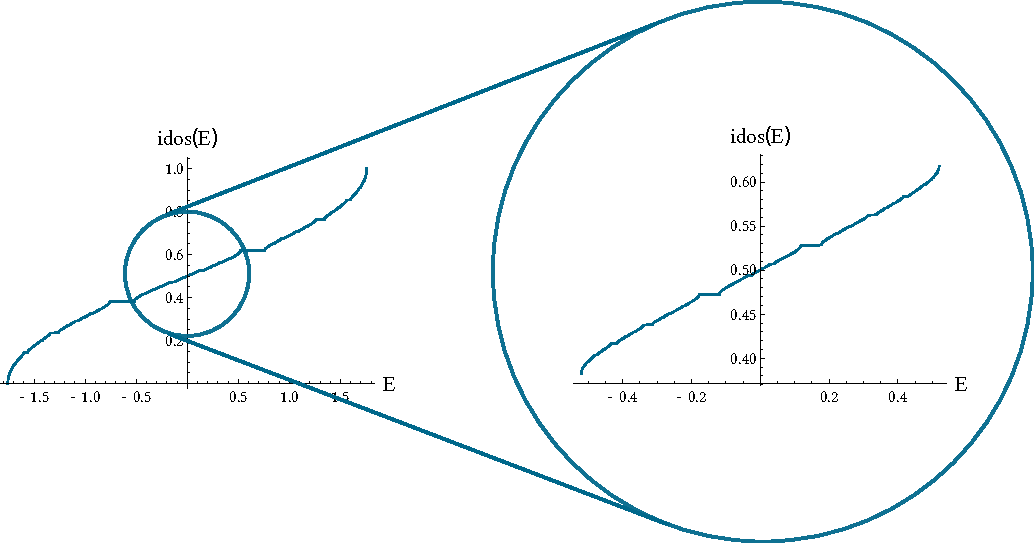
\includegraphics[width=1.\textwidth]{img/3_part2/idos}

	}
	
	\item Eigenstates: (almost all) fractal [Kohmoto \etal{} 83]
\end{itemize}
\>
\<{7cm}{Analytical results}
\begin{itemize}
	\item Gap labeling [Bellissard 86]
	\item Fractal dimensions of the spectrum
	\begin{itemize}
		\item $\rho = t_\A/t_\B \ll 1$: [Piéchon \etal{} 95]
		\item $\rho \sim 1$: [Rüdinger, Sire 96]
	\end{itemize}
	\item Fractal dimensions of the eigenstates, $\rho \ll 1$
	\begin{itemize}
		\item leading order [Thiem, Schreiber 12]
		\item next-to-leading order [Macé \etal{} 16]
	\end{itemize}
\end{itemize}
\>
\)
\end{frame}

\begin{frame}{Fractal dimensions}
\begin{itemize}
	\item $M(L) \propto L^d$ for a non-fractal $d$-dimensional object\dots What happens for a fractal one?
	
	{\centering
	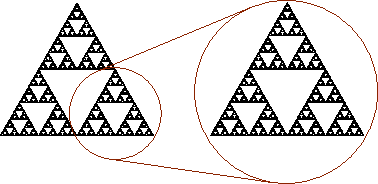
\includegraphics[width=.4\textwidth]{img/2_part1/sierpinski}
	
	{\ss A Sierpiński triangle}
	
	}
	
	\[
		M(L) \sim L^{d_0} \text{, with } d_0 = \log 3/\log 2
	\]
	
	\item $d_0$ is the Hausdorff fractal dimension
	\item $1 < d_0 \simeq 1.58 < 2$, signature of a fractal object
	\item Probe fractality of the $q$ moment of the mass distribution $\to$ generalized fractal dimension $d_q$.
\end{itemize}
\end{frame}

\begin{frame}{The broccoli $E=0$ state}
\(
\<{6cm}
\centering
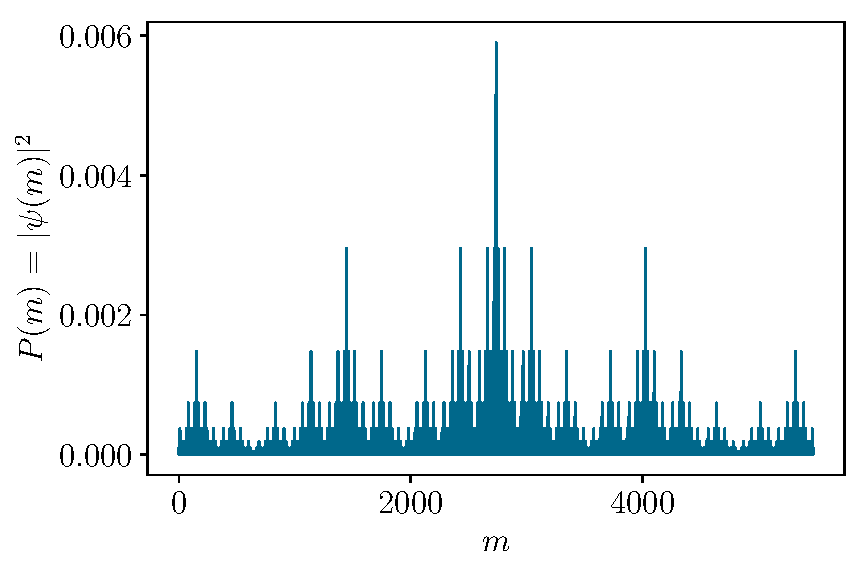
\includegraphics[width=1.\textwidth]{img/2_part1/state_fibo}

{\ss ``Romanesco broccoli'' fractal state at energy $E=0$}
\>
\<{8cm}
\begin{itemize}
	\item State at 0 energy verifies
	\[ t_m \psi(m-1) + t_{m+1}\psi(m+1) = 0 \]
	\item Fibonacci chain decouples into two chains:
	
	{\centering	
	\documentclass[../talk.tex]{subfiles}
\begin{document}


    	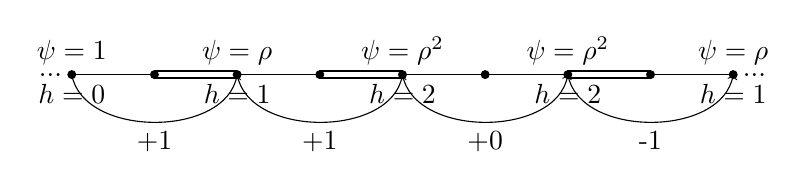
\begin{tikzpicture}[scale=.7]
    		\newcommand{\orig}{-1.5}
    		\newcommand{\trans}{1.5}
    		\newcommand{\vertspac}{-2.}
    		\newcommand{\vertsize}{0} % vertical span of the rectangles
    		\newcommand{\del}{.2}
    		\newcommand{\rad}{2pt} % radii of the circles

    		
    		% set the style of the strong bonds
    		\tikzset{
    			strong/.style={
    				double,
    				double distance=\rad,
    				line width=0.5pt
    				}
    		}
    	
    		% initial chain
    	
    		% bonds 
        	\draw[-] (\orig, 0)  node [left] {...}  -- (\orig+\trans, 0) node [midway, below] {};
			\draw[strong] (\orig+\trans,0) -- (\orig+2*\trans,0) node [midway, below] {};
			\draw[-] (\orig+2*\trans,0) -- (\orig+3*\trans,0) node [midway, below] {};	
			\draw[strong] (\orig+3*\trans,0) -- (\orig+4*\trans,0) node [midway, below] {};
			\draw[-] (\orig+4*\trans,0) -- (\orig+5*\trans,0) node [midway, below] {};
			\draw[-] (\orig+5*\trans,0) -- (\orig+6*\trans,0) node [midway, below] {};
			\draw[strong] (\orig+6*\trans,0) -- (\orig+7*\trans,0) node [midway, below] {};
			\draw[-] (\orig+7*\trans,0) -- (\orig+8*\trans,0) node [right] {...} node [midway, below] {};
    	
    		% sites
			\filldraw (\orig+0*\trans,0) circle (\rad) node [below] {$h=0$} node [above] {$\psi=1$};
			\filldraw (\orig+1*\trans,0) circle (\rad) node [below] {};
			\filldraw (\orig+2*\trans,0) circle (\rad) node [below] {$h=1$} node [above] {$\psi=\rho$};
			\filldraw (\orig+3*\trans,0) circle (\rad) node [below] {};
			\filldraw (\orig+4*\trans,0) circle (\rad) node [below] {$h=2$} node [above] {$\psi = \rho^2$};
			\filldraw (\orig+5*\trans,0) circle (\rad) node [below] {};
			\filldraw (\orig+6*\trans,0) circle (\rad) node [below] {$h=2$} node [above] {$\psi = \rho^2$};
			\filldraw (\orig+7*\trans,0) circle (\rad) node [below] {};
			\filldraw (\orig+8*\trans,0) circle (\rad) node [below] {$h=1$} node [above] {$\psi = \rho$};
			
			% arrow
			\path[->] (\orig+0*\trans,0) edge[bend right = 80] node [below] {+1} (\orig+2*\trans,0);
			\path[->] (\orig+2*\trans,0) edge[bend right = 80] node [below] {+1} (\orig+4*\trans,0);
			\path[->] (\orig+4*\trans,0) edge[bend right = 80] node [below] {+0} (\orig+6*\trans,0);
			\path[->] (\orig+6*\trans,0) edge[bend right = 80] node [below] {-1} (\orig+8*\trans,0);

		\end{tikzpicture}

\end{document}
	}

	\item Work on groups of two letters:
	\begin{itemize}
		\item \ca\cb{} $\leftrightarrow$ R
		\item \cb\ca{} $\leftrightarrow$ L
		\item \ca\ca{} $\leftrightarrow$ U
		\item \cb\cb{} : never occurs
	\end{itemize}
	
\end{itemize}
\>
\)
\end{frame}

\begin{frame}{Structure of the broccoli}
\(
\<{8cm}
\begin{itemize}
	\item Effective chain
	\[
		\underbrace{\ca\cb}_{R}\underbrace{\ca\ca}_{U}\underbrace{\cb\ca}_{L}\underbrace{\cb\ca}_{L}\underbrace{\ca\cb}_{R}\underbrace{\ca\ca}_{U}\dots
	\]
	\item \textbf{Arrow function}: $A(R) = +1$, $A(L) = -1$, $A(U) = 0$.
	\item \textbf{Height function}: $h(m) = \sum_{n \leq m} A_n$
	\item Let $\rho = t_\cb/t_\ca$.
	\[
		\boxed{
		\psi(m) = (-1)^m \rho^{h(m)}
		}
	\]
\end{itemize}
\>
\<{8cm}
\centering
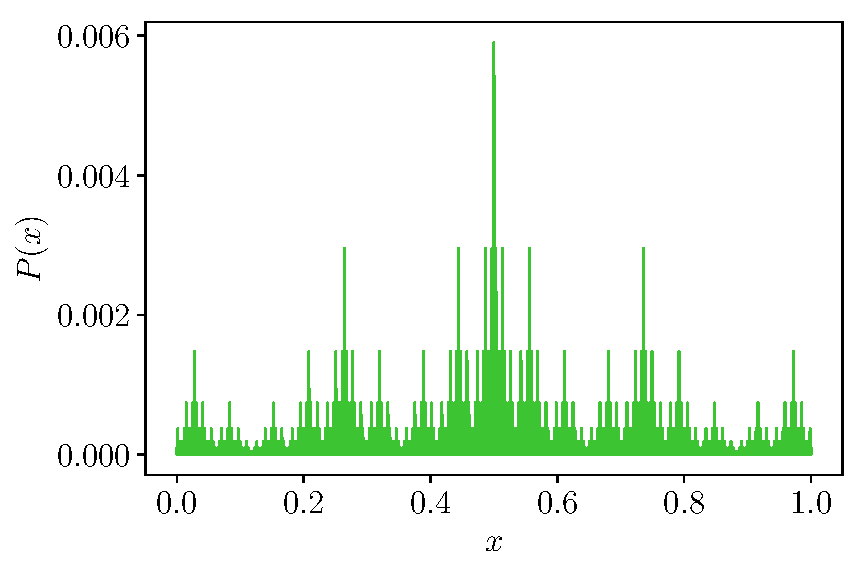
\includegraphics[width=.7\textwidth]{img/2_part1/heights_fibo}

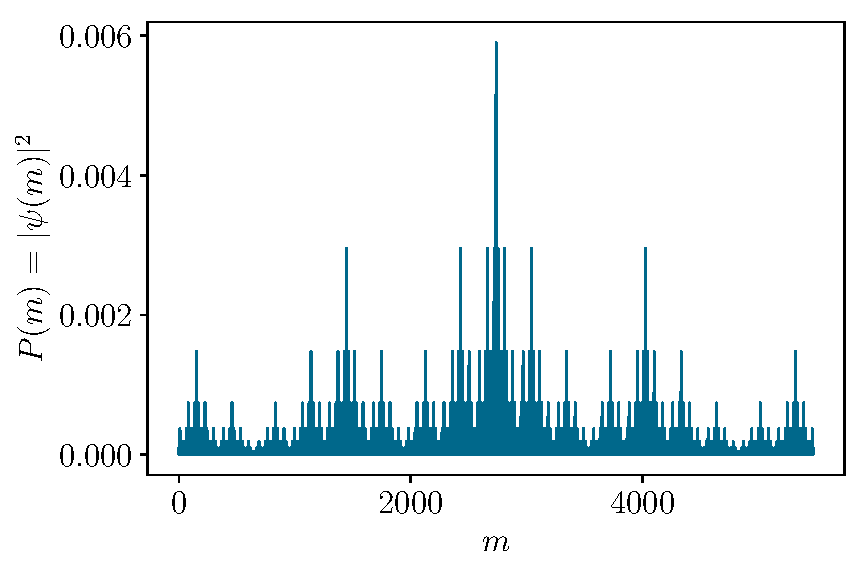
\includegraphics[width=.65\textwidth]{img/2_part1/state_fibo}
\>
\)
\end{frame}

\begin{frame}{Geometry and eigenstate properties}
\(
\<{8cm}
\begin{itemize}
	\item Arbitrary chain \ca\ca\ca\cb\cb\ca\cb\cb\dots{} (not necessarily Fibonacci)
	\item $E=0$ state: $\psi(m) = (-1)^m \rho^{h(m)}$
	\item Geometry $\leftrightarrow$ $h(m)$ function
\end{itemize}

\begin{itemize}
	\item Periodic chain: \ca\ca\ca\ca\ca\dots
%	\documentclass[../talk.tex]{subfiles}
\begin{document}

		\begin{tikzpicture}[scale=.7]
    		\newcommand{\orig}{-1.5}
    		\newcommand{\trans}{1.5}
    		\newcommand{\vertspac}{-2.}
    	
    		% initial chain
    	
    		% bonds 
        	\draw[-] (\orig+\trans,0) -- (\orig+2*\trans,0) node [midway, above] {};
			\draw[-] (\orig+2*\trans,0) -- (\orig+3*\trans,0) node [midway, above] {};	
			\draw[-] (\orig+3*\trans,0) -- (\orig+4*\trans,0) node [midway, above] {};
			\draw[-] (\orig+4*\trans,0) -- (\orig+5*\trans,0) node [midway, above] {};
			\draw[-] (\orig+5*\trans,0) -- (\orig+6*\trans,0) node [midway, above] {};
			\draw[-] (\orig+6*\trans,0) -- (\orig+7*\trans,0) node [midway, above] {};
			\draw[-] (\orig+7*\trans,0) -- (\orig+8*\trans,0) node [midway, above] {};
			\draw[-] (\orig+8*\trans,0) -- (\orig+9*\trans,0) node [midway, above] {};
			
			% wavefunction
			%\draw (\orig+4*\trans,0) -- (\orig+6*\trans,0) node [midway, above] {$\psi(r) = e^{ik r}$};
    	
    		% sites
		    \filldraw (\orig+1*\trans,0) circle (0.05) node [left] {...};
		    \filldraw (\orig+2*\trans,0) circle (0.05) node [below] {};
		    \filldraw (\orig+3*\trans,0) circle (0.05) node [below] {};
		    \filldraw (\orig+4*\trans,0) circle (0.05) node [below] {};
		    \filldraw (\orig+5*\trans,0) circle (0.05) node [below] {};
		    \filldraw (\orig+6*\trans,0) circle (0.05) node [below] {};
		    \filldraw (\orig+7*\trans,0) circle (0.05) node [below] {};
		    \filldraw (\orig+8*\trans,0) circle (0.05) node [right] {};
		    \filldraw (\orig+9*\trans,0) circle (0.05) node [right] {...};
		      
		\end{tikzpicture}
		
\end{document}
	\begin{itemize}
		\item Arrows $= 0 \implies |\psi(m)| = $ cst  
		\item \textbf{extended state}
	\end{itemize}
	\item Disordered chain: \ca\ca\ca\cb\cb\ca\cb\cb\dots
%	%\documentclass[../talk.tex]{subfiles}
%\begin{document}

\begin{tikzpicture}[scale=.7]
    		\newcommand{\orig}{-1.5}
    		\newcommand{\trans}{1.5}
    		\newcommand{\vertspac}{-2.}
    		 \newcommand{\rad}{2pt} % radii of the circles
    		 
    		% set the style of the strong bonds
    		\tikzset{
    			strong/.style={
    				double,
    				double distance=\rad,
    				line width=0.5pt
    				}
    		}
    	
    		% initial chain
    	
    		% bonds 
        	\draw[strong] (\orig+\trans,0) -- (\orig+2*\trans,0) node [midway, above] {};
			\draw[-] (\orig+2*\trans,0) -- (\orig+3*\trans,0) node [midway, above] {};	
			\draw[strong] (\orig+3*\trans,0) -- (\orig+4*\trans,0) node [midway, above] {};
			\draw[strong] (\orig+4*\trans,0) -- (\orig+5*\trans,0) node [midway, above] {};
			\draw[strong] (\orig+5*\trans,0) -- (\orig+6*\trans,0) node [midway, above] {};
			\draw[-] (\orig+6*\trans,0) -- (\orig+7*\trans,0) node [midway, above] {};
			\draw[-] (\orig+7*\trans,0) -- (\orig+8*\trans,0) node [midway, above] {};
			\draw[-] (\orig+8*\trans,0) -- (\orig+9*\trans,0) node [midway, above] {};
			
			% wavefunction
			%\draw (\orig+4*\trans,0) -- (\orig+6*\trans,0) node [midway, above] {$\psi(r) = e^{- r/\xi}$};
    	
    		% sites
		    \filldraw (\orig+1*\trans,0) circle (0.05) node [left] {...};
		    \filldraw (\orig+2*\trans,0) circle (0.05) node [below] {};
		    \filldraw (\orig+3*\trans,0) circle (0.05) node [below] {};
		    \filldraw (\orig+4*\trans,0) circle (0.05) node [below] {};
		    \filldraw (\orig+5*\trans,0) circle (0.05) node [below] {};
		    \filldraw (\orig+6*\trans,0) circle (0.05) node [below] {};
		    \filldraw (\orig+7*\trans,0) circle (0.05) node [below] {};
		    \filldraw (\orig+8*\trans,0) circle (0.05) node [right] {};
		    \filldraw (\orig+9*\trans,0) circle (0.05) node [right] {...};
		      
		\end{tikzpicture}
%\end{document}
	\begin{itemize}
		\item Random arrows $\implies$ $h(m) \simop{m\to\infty} \sqrt{m}$ $\implies |\psi(m)| \sim e^{- \sqrt{m}/\xi}$
		\item \textbf{localized state}
	\end{itemize}
\end{itemize}
\>
\<{8cm}
\begin{itemize}
	\item Quasiperiodic chain
	\begin{itemize}
		\item Discrete scale invariance:
	
		{\centering
		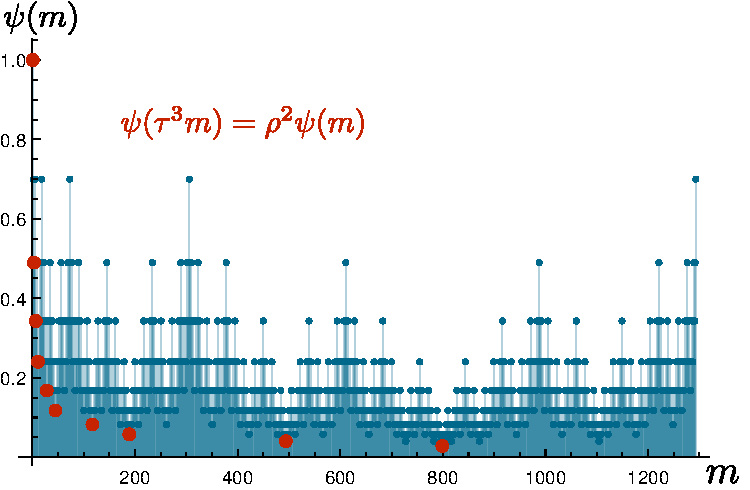
\includegraphics[width=.7\textwidth]{img/2_part1/power_law_decay}}
	
		\item Local power-law behavior $\textcolor{comp}{|\psi(m)| \sim m^{-\alpha}}$
		\item \textbf{critical state} [Kohmoto \etal{} 87]
	\end{itemize}
\end{itemize}
\>
\)
\end{frame}

\begin{frame}{Underlying scale invariance}
Fibonacci chain \emph{itself} scale invariant?

\(
\<{7cm}
\begin{itemize}
	\item Fibonacci words by concatenation:\\
	$C_2 = \lett{AB}$ \\
	$C_3 = \lett{ABA}$ \\
	$C_4 = C_3 C_2 = \lett{ABAAB}$
	
	\item Fibonacci words by \textbf{substitution}:
	\[
		\sub: 
		\begin{cases}
			\A \to \lett{AB}\\
			\B \to \A.
		\end{cases}
	\]
	$C_3 = \lett{ABA}$ \\
	$C_4 = S(C_3) = 
	\only<1>{\sub(\A)\sub(\B)\sub(\A)}
	\only<2>{\lett{AB}\sub(\B)\sub(\A)}
	\only<3>{\lett{AB}\A\sub(\A)}
	\only<4>{\lett{AB}\A\lett{AB}}
	$
\end{itemize}
\>
\<{7cm}
\begin{itemize}
	\item Infinite chain = fixed point of the substitution: \\
	$S(\lett{ABAAB}\dots) = \lett{ABAAB}\dots$
	\item Geometric substitution:
	
	{\centering
	    	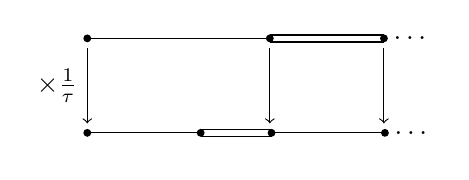
\begin{tikzpicture}[scale=.6]
    		\newcommand{\orig}{-1.5}
    		\newcommand{\s}{1.5} % length of short bonds
    		\renewcommand{\L}{2.4} % length of long bonds
    		\newcommand{\golden}{1.61}
    		\newcommand{\rs}{\golden*\s} % length of renormalized short bonds
    		\newcommand{\rL}{\golden*\L} % length of renormalized long bonds
    		\newcommand{\vertspac}{2.}    		
    		\newcommand{\rad}{2pt} % radii of the circles
    		\newcommand{\del}{0.2}
    		
    		% set the style of the strong bonds
    		\tikzset{
    			strong/.style={
    				double,
    				double distance=\rad,
    				line width=0.5pt
    				}
    		}
    	
    		%%%%%%%%%% initial chain
    		% bonds 
			\draw[-] (\orig,\vertspac) -- (\orig+\rL,\vertspac) node [midway, below] {$\A$};
			\draw[strong] (\orig+\rL,\vertspac) -- (\orig+\rs+\rL,\vertspac) node [midway, below] {$\B$};	
    		% sites
		    \filldraw (\orig,\vertspac) circle (\rad);% node [below] {6};
		    \filldraw (\orig+\rL,\vertspac) circle (\rad);% node [below] {3};
		    \filldraw (\orig+\rs+\rL,\vertspac) circle (\rad) node [right] {\dots};% node [below] {8};
		        
    		%%%%%%%%% renormalized chain
    		% bonds 
			\draw[-] (\orig,0) -- (\orig+\L,0) node [midway, below] {$\A$};
			\draw[strong] (\orig+\L,0) -- (\orig+\s+\L,0) node [midway, below] {$\B$};	
			\draw[-] (\orig+\s+\L,0) -- (\orig+\s+2*\L,0) node [midway, below] {$\A$};
%			\draw[-] (\orig+2*\s+2*\L,0) -- (\orig+2*\s+3*\L,0) node [midway, below] {$\A$};
%			\draw[strong] (\orig+2*\s+3*\L,0) -- (\orig+3*\s+3*\L,0) node [midway, below] {$\B$};
%			\draw[-] (\orig+3*\s+3*\L,0) -- (\orig+3*\s+4*\L,0) node [midway, below] {$\A$};
%			\draw[strong] (\orig+3*\s+4*\L,0) -- (\orig+4*\s+4*\L,0) node [midway, below] {$\B$};
    	
    		% sites
		    \filldraw (\orig,0) circle (\rad);% node [below] {6};
		    \filldraw (\orig+\L,0) circle (\rad);% node [below] {3};
		    \filldraw (\orig+\s+\L,0) circle (\rad);% node [below] {8};
		    \filldraw (\orig+\s+2*\L,0) circle (\rad) node [right] {\dots};% node [below] {5};
%		    \filldraw (\orig+2*\s+3*\L,0) circle (\rad);% node [below] {2};
%		    \filldraw (\orig+3*\s+3*\L,0) circle (\rad);% node [below] {7};
%		    \filldraw (\orig+3*\s+4*\L,0) circle (\rad);% node [below] {4};
%		    \filldraw (\orig+4*\s+4*\L,0) circle (\rad);% node [below] {1};

		    % arrows below rectangles
		    \draw [<-] (\orig,\del) -- (\orig,\vertspac-\del) node [midway, left] {$\times \frac{1}{\tau}$};
		    \draw [<-] (\orig+\rL,\del) -- (\orig+\rL,\vertspac-\del);
		    \draw [<-] (\orig+\rs+\rL,\del) -- (\orig+\rs+\rL,\vertspac-\del);
		      
		\end{tikzpicture}
	}
	
	\item \textbf{Infinite chain scale invariant}, scaling factor $1/\tau$.
	
\end{itemize}
\>
\)
\end{frame}

\begin{frame}{Height distribution \& multifractality}
\(
\<{7cm}
Partition function of the heights:
\[
	Z_L(\beta) = \sum_{m \in \reg(L)} e^{-\beta h(m)}
\]
Substitution $\to$ scaling law behavior:
\[
	Z_L(\beta) \simop{L \to \infty} L^{\omega(\beta)}
\]
with
\[
	\om(\beta) = \frac{\sinh^{-1}(1+\cosh(\beta))}{2+\sqrt{5}}
\]
$\to$ access to the distribution of heights
\>
\<{7cm}
Height grows slowly:
\[
	h_\text{typ}(L) \sim \sqrt{\log L}
\]

Fractal dimensions of the $E=0$ state:
\[
	d_q = \frac{q \om(2\kappa) - \om(2\kappa q)}{q-1},~\text{with }\kappa = |\log \rho|
\]
$0 < d_q < 1$ $\to$ \textbf{fractal state}

\flushright{[Macé \etal{} 17]}
\>
\)

\end{frame}

\begin{frame}{Beyond quasiperiodicity}
\(
\<{7cm}
\(
\<{4cm}
B3 chain:
\[
	\sub: 
	\begin{cases}
		\A \to \lett{ABBB}\\
		\B \to \A.
	\end{cases}
\]

Unbounded fluctuations

$\to$ \textbf{not quasiperiodic}

[Frank, Robinson 08]
\>
\<{3cm}
\centering
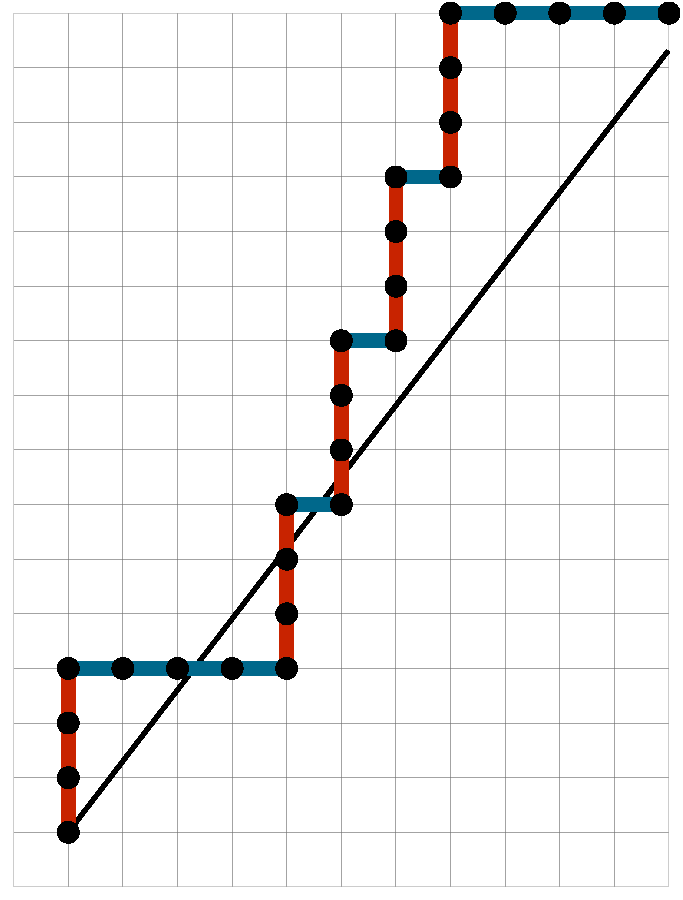
\includegraphics[width=1.\textwidth]{img/2_part1/CP_b3_cut}
\>
\)
\>
\<{7cm}

{\centering
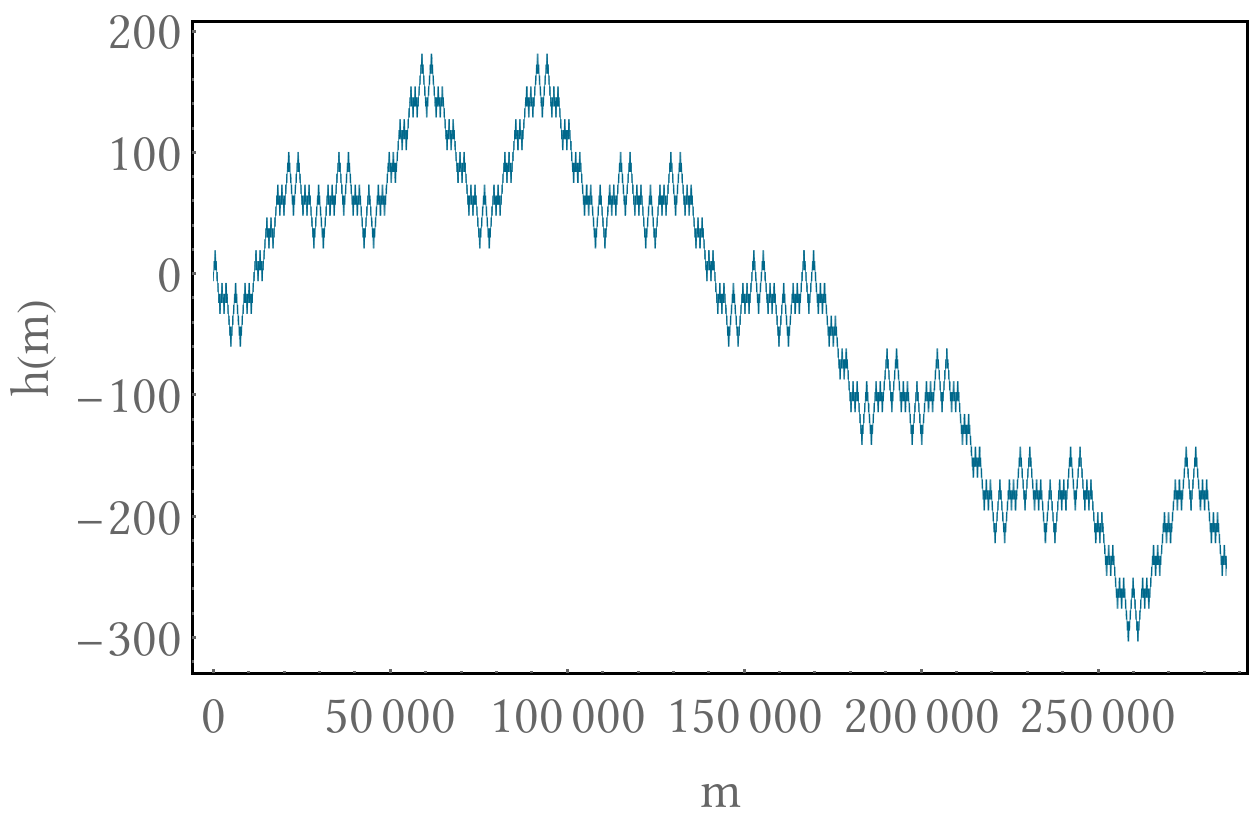
\includegraphics[width=.7\textwidth]{img/2_part1/7_height_b3}

}

Height: power-law growth [Dumont 89]
\[
h(m) = C(m)m^\alpha
\]
%$C$: log-periodic function.

$\to$ \textbf{non-fractal, localized state}
\[
	|\psi(m)| \simop{m \to \infty} e^{-m^\alpha/\xi}
\]
\>
\)
\end{frame}

\begin{frame}{Conclusions}
$E=0$ state of \textcolor{BostonBlue}{two}-\textcolor{comp}{letters} tight-binding chains:
\begin{itemize}
	\item Height field $h(m)$ $\to$ $\psi(m) = (-1)^m \rho^{h(m)}$
\end{itemize}
Effect of the (dis)order:
\begin{itemize}
	\item \textbf{Periodic} $\to$ no height growth $\to$ \textbf{extended} state
	\item \textbf{Quasiperiodic} $\to$ slow height growth ($h(L) \sim \sqrt{\log L})$ $\to$ critical, \textbf{fractal} state
	\item \textbf{Random}/deterministic non-qp $\to$ fast height growth ($h(L) \sim L^\alpha$) $\to$ \textbf{localized} state
\end{itemize}
\end{frame}
